\section{数据结构}
针对图像文件在管理系统中的特性,以及考虑到图像在卷积神经网络中的加载方式,我们采取的管理并储存图像的方式是线性表和链表。

\subsection{线性表}
在线性表中,我们储存的是每个图片在计算机中的地址,由地址对于具体的图片进行管理。在使用CNN网络进行学习的时候,通过传入地址读取具体的图片,并且对于图片进行学习。因此,我们实现了以下的特殊方法:初始化、迭代、求长度;以及以下的自定义方法:返回匹配项下标、添加元素、删除元素、插入元素、查找元素。\\

\noindent LinearTable 类:表示线性表,包含以下主要功能:

\noindent \_\_init\_\_(self):初始化一个空的线性表,使用列表 datalist 存储数据。

\noindent \_\_iter\_\_(self):使线性表可迭代,可以直接迭代线性表中的元素。

\noindent \_\_len\_\_(self):返回线性表中元素的数量。

\noindent index(self, data):返回第一个匹配项的下标,如果不存在则返回 -1。

\noindent add\_data(self, data):向线性表末尾添加一个新的数据项。

\noindent find\_data(self, data):查找线性表中所有匹配指定数据项的下标,返回一个列表。

\noindent insert\_data(self, location, data):在指定位置插入新的数据项。

\noindent delete\_data(self, data):从线性表中删除第一个匹配指定数据项的元素。

\subsection{双向链表}
在LinkedList.py中,我们实现了一个基本的双向链表结构,用于管理图像文件的路径。以下是每个类的主要功能:\\

\noindent ImageNode 类:表示链表中的节点,每个节点包含一个图像文件的路径。节点还包括指向下一个节点和上一个节点的指针。

\noindent ImageLinkedList 类:表示双向链表,包含以下主要功能:

\noindent add\_image(image\_path):向链表末尾添加一个新的图像节点。

\noindent delete\_image(image\_path):从链表中删除包含指定图像路径的节点。

\noindent search(image\_path):在链表中查找包含指定图像路径的节点,返回该节点。

\noindent is\_empty():检查链表是否为空。

\noindent length():返回链表中节点的数量。

\noindent display\_images():打印链表中所有图像节点的路径。

\noindent \_\_getitem\_\_(index):通过索引获取链表中特定位置的图像路径。

\noindent to\_list():将链表中的元素输入到列表中并返回

\subsection{数据加载与测量}
与数据结构和数据加载相关的文件是dshwwithpytorch文件夹中的datawithlt.py和datawithll.py文件,前者是使用线性表,后者是使用链表。\\

在这两个文件中,对数据进行了加载和预处理,并在这个过程中调用了例如time()对于加载时间进行测量,以及导入psutil包对于内存进行测量。直接运行这两个文件夹即可得到初步的结果如下。

\begin{figure}[H]
	\centering
	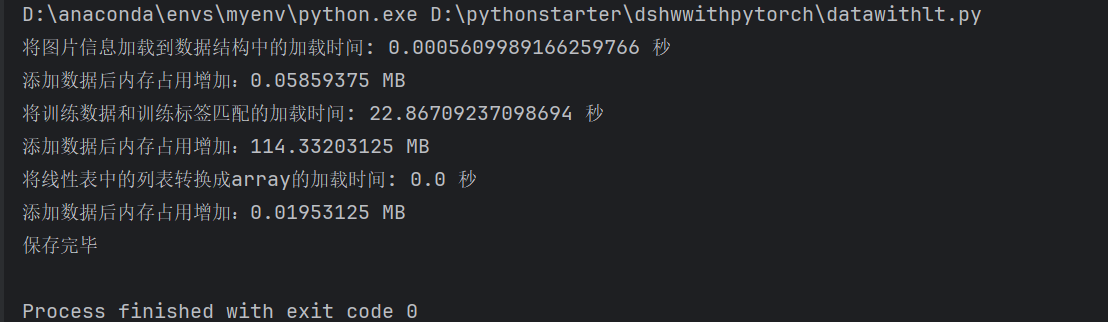
\includegraphics[width=0.8\textwidth]{lt.png}  % 替换为你的图片文件名
	\caption{线性表的运行时间和占用内存}
	\label{fig:example}
\end{figure}

\begin{figure}[H]
	\centering
	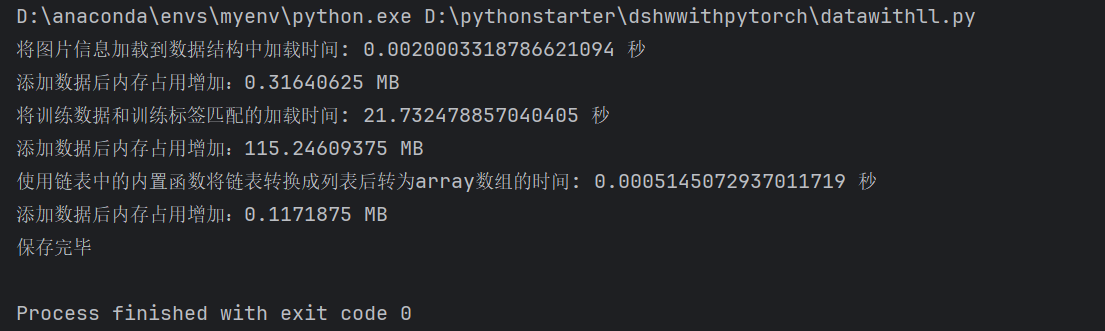
\includegraphics[width=0.8\textwidth]{ll.png}  % 替换为你的图片文件名
	\caption{链表的运行时间和占用内存}
	\label{fig:example}
\end{figure}

\subsection{定量分析}
\subsubsection{方法和评价标准}
在实验中,为了定量分析,准确起见,我将每个数据结构加载了十二次,比较不同的数据结构在不同的指标上的差别,并分析出现这样的结果的原因。与之相关的文件是dshwwithpytorch文件夹里面的comparell.py,comparelt.py,myplot.py,time\&memory文件夹和plots文件夹。在comparell.py,comparelt.py两个文件中我分别用两种数据结构运行了12次,获得实验数据。而后我将数据以列表的形式储存到time\&memory文件夹中。\\

最后,我在myplot.py文件中绘制了比较的图像,而后将图像导出保存至plots文件夹中。分析的指标分为三个进程,共有六个,三个为时间指标,三个为内存指标。它们是:(1)将图片信息加载到数据结构中的加载时间和添加数据后内存占用。(2)将训练数据和训练标签匹配的加载时间和内存占用。(3)将各个数据结构中的数据转换成array数组的加载时间和内存占用。在实验时选取的数据集是训练集。

选择这三项进程的六个指标原因如下。\\

首先,由于创建数据结构的目的就是储存、管理数据,因此选择将图片信息加载到数据结构中的加载时间和添加数据后内存占用是非常自然的事情。\\

其次,由于分类问题需要将数据和标签匹配,因此数据结构在匹配的速度和占用内存大小的性能就成为了评价数据结构的重要指标。\\

最后,不管什么数据结构,由于神经网络只能接受特定的数据类型,因此我们都需要将数据结构中的数据转换数据类型后才能进行学习,因此我们选择了将数据结构中的数据转换成array数组的加载时间和内存占用作为两个评价指标。
\subsubsection{将图片信息加载到数据结构中的加载时间和内存占用}
\begin{figure}[H]
	\centering
	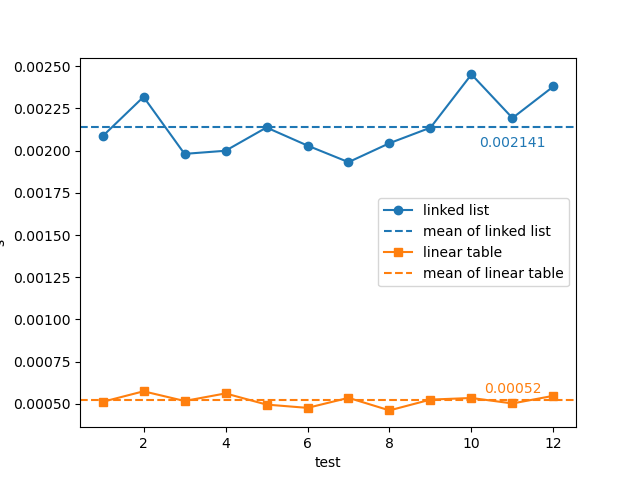
\includegraphics[width=0.7\textwidth]{time1}  % 用于插入图片的命令
	\caption{将图片信息加载到数据结构中的加载时间}
	\label{fig:your_label}
\end{figure}
\begin{figure}[H]
	\centering
	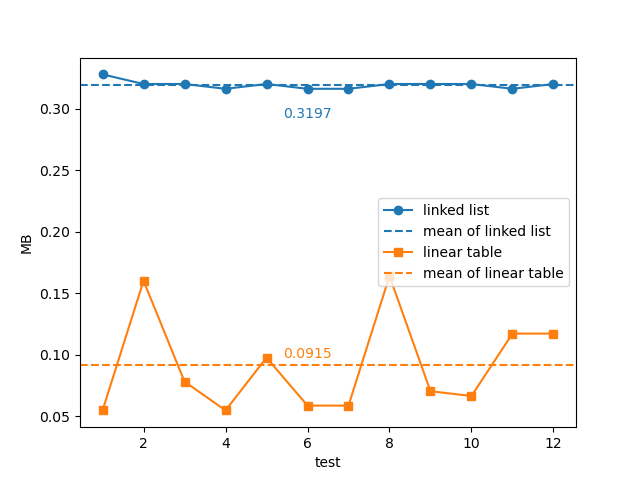
\includegraphics[width=0.7\textwidth]{memory1}  % 用于插入图片的命令
	\caption{将图片信息加载到数据结构中的内存占用}
	\label{fig:your_label}
\end{figure}
根据图表可以看出,从时间上来看,链表花费的时间是线性表的4倍左右,链表占用的内存是线性表的3倍左右。据分析,这样的结果产生的原因是在加载阶段,链表的每一个节点要比线性表多创建了头指针和尾指针,因此不管是加载时间还是占用内存,链表都比线性表要花更多的时间。
\subsubsection{将训练数据和训练标签匹配的加载时间和内存占用}
\begin{figure}[H]
	\centering
	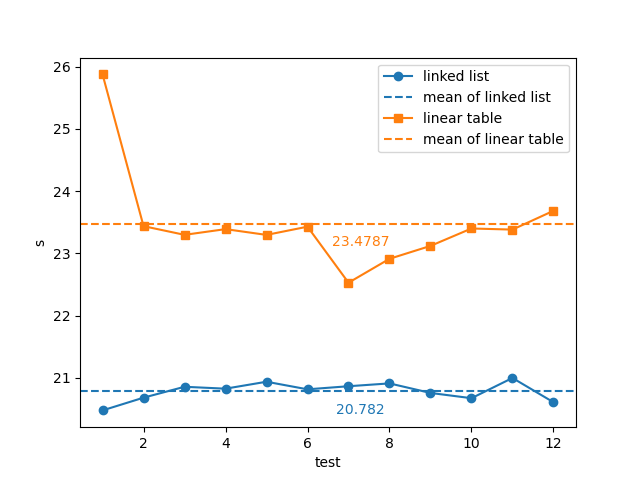
\includegraphics[width=0.7\textwidth]{time2}  % 用于插入图片的命令
	\caption{将训练数据和训练标签匹配的加载时间}
	\label{fig:your_label}
\end{figure}
\begin{figure}[H]
	\centering
	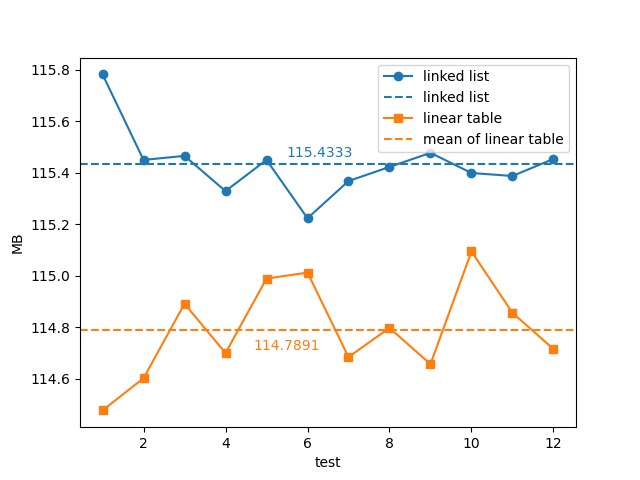
\includegraphics[width=0.7\textwidth]{memory2}  % 用于插入图片的命令
	\caption{将图片信息加载到数据结构中的内存占用}
	\label{fig:your_label}
\end{figure}
在这两个指标中,链表的加载时间普遍低于线性表,内存占用普遍高于线性表,但是差别并不明显。原因可能链表可以动态开辟存储空间,因此在匹配的过程中时间较短,但是由于每个节点都有指针,因此总体内存增大。
\subsubsection{将各个数据结构中的数据转换成array数组的加载时间和内存占用}
\begin{figure}[H]
	\centering
	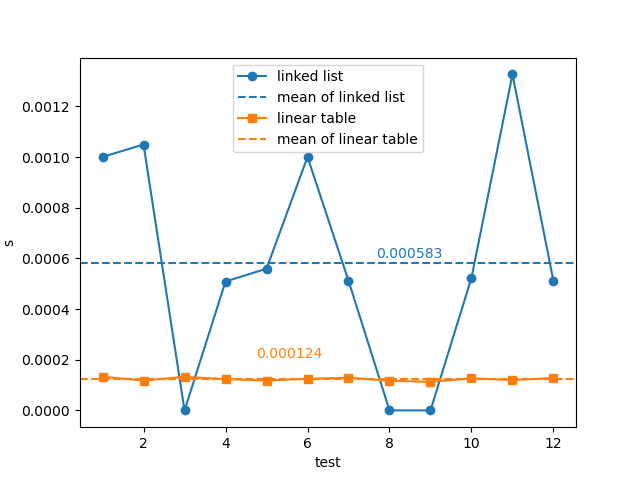
\includegraphics[width=0.7\textwidth]{time3}  % 用于插入图片的命令
	\caption{将各个数据结构中的数据转换成array数组的加载时间}
	\label{fig:your_label}
\end{figure}
\begin{figure}[H]
	\centering
	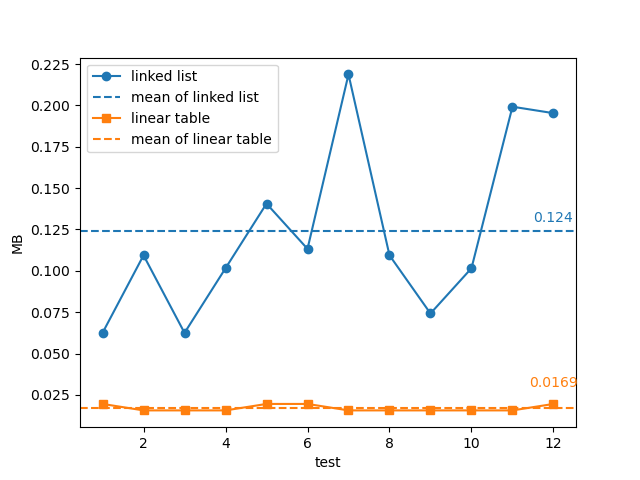
\includegraphics[width=0.7\textwidth]{memory3}  % 用于插入图片的命令
	\caption{将图片信息加载到数据结构中的内存占用}
	\label{fig:your_label}
\end{figure}
在转换数组的这两个指标中,链表的加载时间是线性表的6倍左右,占用内存是线性表的7倍。原因应当如下:线性表在储存信息的时候就是采取的列表形式,因此按照线性表的顺序逐一转换即可;而链表由于分散储存,因此需要在链表中写一个转换成线性表的函数,才能将链表中的元素先储存进一个列表中,而后才能进一步转换为数组。

\subsection{误差}
首先在实验的时候犯了一个错误,如图是将训练数据和训练标签匹配的加载时间的图像。从图中可以看出,第一次实验后内存便基本为零了。猜想的原因是,线性表的实验过程中是用for循环进行实验的,但是可能在这个过程中需要清空内存,但是没有清空,于是就出现了这样的情况。
\begin{figure}[H]
	\centering
	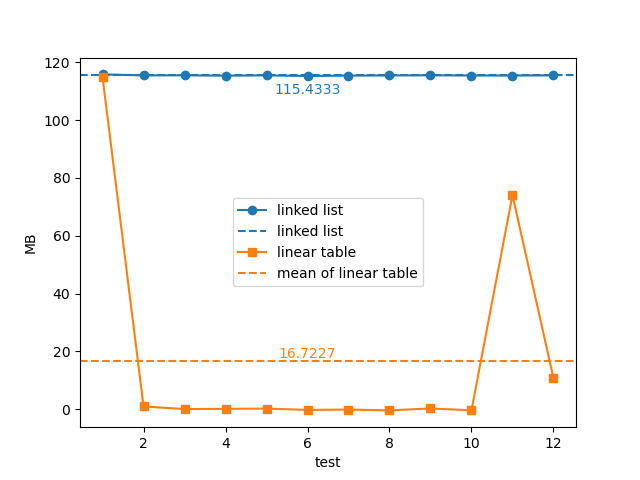
\includegraphics[width=0.7\textwidth]{wrong1}  % 用于插入图片的命令
	\caption{错误图样}
	\label{fig:your_label}
\end{figure}
因此保险起见,我后来分别将线性表和链表的单次实验进行了12次,并手动将数据储存进线性表中。原始数据可以在comparell.py和comparelt.py中看到,也就是上面几节中图片展示的样子。但是明显可以看出,有的数据波动过大,例如2.4.4节中的图7,图8,目前并不是很清楚原因是什么。\\

另外,在实验过程中偶尔会出现时间或内存为0.0的状况,时间为0.0的原因应该是使用了time包中的time()函数进行计时,后来换成perf\_counter()函数后就不会出现这样的状况了。





